\subsection{Künstliche Neuronale Netze (ANN)}
\label{ann}
Können eingesetzt werden für 
\begin{itemize}
    \item überwachtes Lernen
    \item unüberwachtes Lernen
    \item Reinforcement Learning
\end{itemize}

\underline{Idee}: Komplexe Lernaufgabe wird durch viele versteckte Schichten in Teilaufgaben zerlegt. Vorteil dabei ist, dass die beim Lernalgorithmus beim Lernen der Gewichte auch selbst entscheidet, welche Zwischenkonzepte die Schichten repräsentieren $\rightarrow$ \emph{feature-engineering} (manuelle Definition der Merkmale) entfällt.\\

\emph{Feedforward}-Netzwerk: \emph{Input Layer} nimmt Eingebewerte entgegen, \emph{Output Layer} gibt Ausgabewerte aus. Dazwischen liegen \emph{Hidden Layer}, die die Eingabewerte transformieren. Ab 2 Hidden-Layern spricht man von einem \emph{Deep Neural Network}. Die einzelnen Neuronen sind in Schichten angeordnet, wobei jedes Neuron mit jedem Neuron der vorherigen Schicht \emph{gewichtet} verbunden ist.
Über die \emph{Aktivierungsfunktion} (nimmt die gewichteten Werte vorheriger Neuronen sowie einen \emph{Bias-Wert} entgegen) wird die Ausgabe eines Neurons bestimmt.
Evaluiert wird das Netzwerk über eine \emph{Verlustfunktion}, die den Fehler zwischen den Ausgaben des Netzwerks und den tatsächlichen Ausgaben berechnet.\\

\underline{\textbf{Aktivierungsfunktionen}}:\\
Die \emph{Aktivierungsfunktion} ist typischerweise in allen \emph{Hidden-Layern} gleich; im Ausgabelayer aber anwendungsabhängig und üblicherweise nicht identisch mit denen der Hidden-Layer (Regression: Ausgabe muss gesamte reellen Zahlen als Wertebereich haben; Klassifikation: Bool'sche Ausgabe (wenn binär) oder eine Wahrscheinlichkeit, ggf. auch mehrere Ausgabeneuronen für einzelne Klassen).

\begin{center}
    \begin{tabular}{c|c|c|c|c}
        \textbf{Funktion} & \textbf{Formel} & \textbf{Ableitung} & \textbf{Eigenschaften}&\textbf{Verlauf}\\
        \hline
        Threshold & \makecell{$h^{\text{thresh}}(x)=$\\$\begin{cases}1 & \text{für } x\geq 0\\0 & \text{für } x<0\end{cases}$} & nicht differenzierbar & Praxis (-)&\makecell{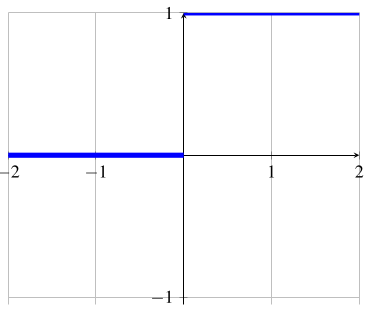
\includegraphics[width=0.15\textwidth]{deepLearning/h_tresh.png}}\\
        \hline
        Identität & $h^{\text{id}}(x)=x$ & $h^{\text{id}}(x)'=1$ & \makecell{Praxis (-);\\nur im Output bei\\Regression}&\makecell{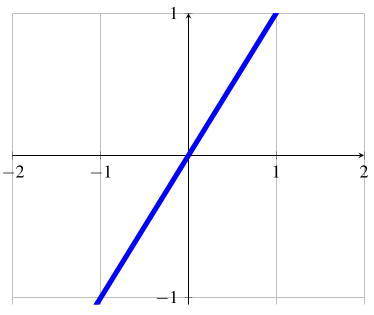
\includegraphics[width=0.15\textwidth]{deepLearning/h_id.png}}\\
        \hline
        Sigmoid & $h^{\text{logit}}(x)=\frac{1}{1+e^{-x}}$ & \makecell{$h^{\text{logit}}(x)'=$\\$h^{\text{logit}}(x)(1-h^{\text{logit}}(x))$} & \makecell{$h^{\text{logit}}(x)\in [0,1]$\\$\rightarrow$ bin. Klassifikat.} & \makecell{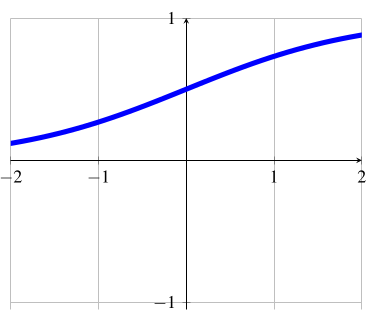
\includegraphics[width=0.15\textwidth]{deepLearning/h_logit.png}}\\
        \hline
        Hyperbol. Tangent & $h^{\text{tanh}}(x)=\frac{e^x-e^{-x}}{e^x+e^{-x}}$ & \makecell{$h^{\text{tanh}}(x)'=$\\$1-(h^{\text{tanh}}(x))^2$} & $h^{\text{tanh}}(x)\in [-1,1]$ & \makecell{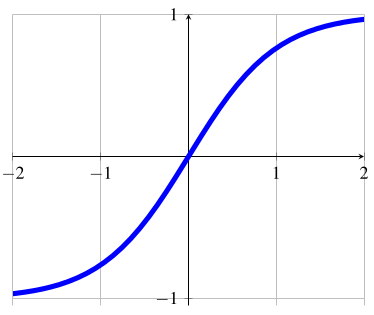
\includegraphics[width=0.15\textwidth]{deepLearning/h_tanh.png}}\\
        \hline
        \makecell{Rectified\\Linear Unit} & $h^{\text{ReLU}}(x)=\max(0,x)$ & \makecell{$h^{\text{ReLU}}(x)'=$\\$\begin{cases}0 & \text{für } x<0\\1 & \text{für } x\geq 0\end{cases}$} & $h^{\text{ReLU}}(x)\in [0,\infty)$ & \makecell{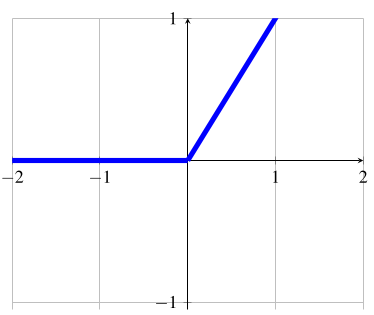
\includegraphics[width=0.15\textwidth]{deepLearning/h_relu.png}}\\
        \hline
        Softmax & & & \multicolumn{2}{c}{\makecell{$h^{\text{smax}}(x_i)\in [0,1]$\\$\sum_{i=1}^{n}h^{\text{smax}}(x_i)=1$\\$\rightarrow$ Mehrklassenklassifikation}} \\
    \end{tabular}
\end{center}

\underline{\textbf{Kosten-/Verlustfunktionen}}:\\

\begin{center}
    \begin{tabular}{c|c|c|c}
        \textbf{Funktion} & \textbf{Formel} & \textbf{Ableitung} & \textbf{Eigenschaften}\\
        \hline
        Quadratischer Fehler & \makecell{$L^{\text{qF}}(D,f)=$\\$\sum_{i=1}^{m}(f(x^{(i)})-y^{(i)})^2$} & $L'(D,f)=2(f(x)-y)$ & für $h^{\text{id}}$\\
        \hline
        Logistische Kosten & \makecell{$L^{\text{logit}}(D,f)=$\\$-\sum_{i=1}^{m}[y^{(i)}\ln(f(x^{(i)}))$\\$+(1-y^{(i)})\ln(1-f(x^{(i)}))]$} & $L'(D,f)=f(x)-y$ & \makecell{für $h^{\text{logit}}$\\ oder $h^{\text{ReLU}}$}\\
    \end{tabular}
\end{center}


Bei Verwendung der Identitätsfunktion $h^{\text{id}}=x$ als Aktivierungsfunktion und dem quadratischen Fehler $L^{\text{qF}}$ als Verlustfunktion ist die Ausgabe äquivalent zu der optimal angepassten linearen Funktion für die \underline{lineare Regression}.\\

Bei Verwendung der Sigmoid-Funktion $h^{\text{logit}}$ als Aktivierungsfunktion und der logistischen Kostenfunktion $L^{\text{logit}}$ ist die Ausgabe äquivalent zu dem optimalen Modell der \underline{logistischen Regression}.\\

\underline{\textbf{Backpropagation}}:\\
\begin{figure}[H]
    \centering
    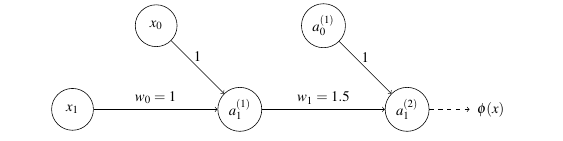
\includegraphics[width=1\textwidth]{deepLearning/EinfachesANN.png}
    \caption{Ausgangsbeispiel mit $x_1=0.1$, $x_2=0.2$, $a_0^{(1)}=0.05$, $y=0.3$, $act=\text{ReLU}$, $L^{\text{logit}}$ und $\gamma=0.1$}
\end{figure}

\emph{\textbf{1. Forward-Pass}}: Berechne die Ausgabe des Netzes für einen gegebenen Eingabevektor $x \rightarrow$ Netzwerk von Input bis Output unter Berücksichtigung von Gewichten, Bias und Aktivierungsfunktionen durchrechnen.
\begin{equation*}
    \begin{aligned}
        \boldsymbol{z_1^{(1)}} = w_0x_1+1x_0=1\cdot0.2+0.1=0.3 &\longrightarrow \boldsymbol{a_1^{(1)}}=h^{relu}(z_1^{(1)}) = \max \left[ 0, 0.3\right] = 0.3\\
        \boldsymbol{z_1^{(2)}} = w_1a_1^{(1)}+1a_0^{(1)}=1.5\cdot0.3+0.05=0.5 &\longrightarrow \boldsymbol{a_1^{(2)}}=h^{relu}(z_1^{(2)}) = \max \left[ 0, 0.5\right] = 0.5 = \boldsymbol{\varPhi(x)}\\
    \end{aligned}
\end{equation*}\\

\emph{\textbf{2. Kosten- und Fehlerberechnung}}: Berechne den Fehler des Netzes durch die Verlustfunktion $L$; beginne beim Output-Layer und rechne nach vorne.
\begin{equation*}
    \begin{aligned}
        \boldsymbol{cost(y, a_1^{2})}  &= -(y\ln(a_1^{(2)})+(1-y)\ln(1-a_1^{(2)})) = -(0.3\cdot-0.693+0.7\cdot-0.693) = 0.693
    \end{aligned}
\end{equation*}

Berechnung des Fehlers im linearen Anteil des \underline{Output-Layers} durch:
\begin{equation*}
    \begin{aligned}
        \boldsymbol{\delta(z_j^{(k)})}  &= \frac{\partial cost(y, a_1^{(2)})}{\partial z_1^{(2)}}
    \end{aligned}
\end{equation*}

$\rightarrow$ Aktivierungsfunktion in Kostenfunktion einsetzen und nach $z_1^{(2)}$ ableiten.\\

Wenn Kostenfunktion $=L^\text{logit}$ (Logistische KF) \underline{und} Aktivierungsfunktion $=h^\text{logit}$ (Sigmoid), gilt $\delta(z_i^{(l)})=a_i^{(l)}-y_i$.

Der Fehler im linearen Anteil $\delta(z_1^{(2)})$ der \underline{Hidden Layer} ist gegeben durch:
\begin{equation*}
    \begin{aligned}
        \boldsymbol{\delta(z_j^{(k)})}  &= \text{act}'(z_j^{(k)})\cdot\sum_{i=1}^{n_{k+1}}\delta(z_i^{(k+1)})\cdot w_{ij}^{(k+1)}
    \end{aligned}
\end{equation*}

Fehler eines Neurons berechnet sich aus dem Produkt von
\begin{itemize}
    \item linearer Wert des aktuellen Neurons ($z_j^{(k)}$) eingesetzt in die Ableitung der Aktivierungsfunktion
    \item Summe der Fehler der Neuronen der nächsten Schicht multipliziert mit den Gewichten der Verbindung zu diesen Neuronen\\
\end{itemize}

\emph{\textbf{3. Neuberechnung der Gewichte}}: Berechne die neuen Gewichte durch Anpassung der alten Gewichte um den Fehler zu minimieren.
\begin{equation*}
    \begin{aligned}
        \boldsymbol{w_{ij}^{(k)_\text{neu}}}  &= w_{ij}^{(k)_\text{alt}}-\gamma\cdot\delta(z_j^{(k)})\cdot a_i^{(k-1)}
    \end{aligned}
\end{equation*}

Neues Gewicht ergibt sich aus dem alten Gewicht abzüglich des Produkts aus
\begin{itemize}
    \item Lernrate $\gamma$
    \item Fehler des Neurons
    \item Ausgabe des Neurons der vorherigen Schicht\\
\end{itemize}

\emph{\textbf{4. Wiederhole 1.-3. Schritt}}: Forward-Pass, Neuberechnung des Fehlers und ggf. weitere Backpropagation zur Modellverbesserung\\

\underline{\textbf{Auswahl des Trainingsdatensatzes}}: Gradient Descent mit gesamtem Datensatz kann u.U. sehr langsam sein, wenn $D$ sehr groß ist. Alternativen:
\begin{itemize}
    \item \emph{Stochastic Gradient Descent (SGD)}: Berechne den Fehler und die Gewichtsanpassung anhand eines zufällig gewählten Datenpunktes
    \begin{itemize}
        \item Vorteil: schnelleres Lernen
        \item Nachteil: ungenaue Schätzung des Gradienten $\rightarrow$ nächstes lokales Minimum wird nicht zielstrebig angesteuert, Gesamtkosten können während des Lernens stark schwanken, keine Parallelisierbarkeit
    \end{itemize}
    \item \emph{Mini-Batch Gradient Descent (MBGD)}: Berechne den Fehler und die Gewichtsanpassung anhand einer zufällig gewählten Teilmenge des Datensatzes. Kompromiss zwischen SGD und GD mit geringerem Fluktuationsgrad. Parallelisierbarkeit indem die Batchgröße entsprechend der Anzahl zu Verfügung stehender Rechenkerne gewählt wird.
\end{itemize}

\underline{\textbf{Auswahl der Aktivierungsfunktion}}: Ableitung der Aktivierungsfunktion ist Bestandteil des Algorithmus. Bestimmte Funktionen können zu Problemen führen, wenn bei bestimmten (x)-Werten die Ableitung gegen 0 geht (z.B. Sigmoid-Funktion bei $x\geq3 \text{ oder } x\leq-3\rightarrow<0.1$; sog. \emph{vanishing gradient problem}). Ähnlich: \emph{Exploding Gradient Problem} bei Werten $>1$. Lösung: ReLU-Aktivierung, da für $x>0$ die Ableitung von $h^{relu}=1$ und damit gedeckelt. Nachteil: für $x<0$ ist die Ableitung stets $0\rightarrow$ Lösung durch Verwendung von \emph{splus}.